% -*- coding=utf-8 -*-
%%%%%%%%%%%%%%%%%%%%%%%%%%%%%%%%%%%%%%%%%%%%%%%%%%%%%%%%%%%%%%%%%%%%%%%%%%%%%%%%%%%%%%%%%%%%%%%
%   河南中医药大学本科生毕业论文LaTeX模板
%   声明:本模板是在陕西师范大学本科生毕业论文模板的基础上进行修改得来的,非常感谢原作者提供的模板
%   原模板见:https://www.overleaf.com/latex/templates/shan-xi-shi-fan-da-xue-ben-ke-sheng-bi-ye-lun-wen-texmo-ban/rkxzpttqqzyt
%   使用要求:
%       编译器:XeLatex(2019+),建议关闭拼写检查
%       或者直接使用overleaf
%   使用方法:
%       编辑/tex目录下的各个tex文件的文件内容
%       最后编译main.tex
%       警告:需要修改配置就编辑main.tex的内容,编辑内容去/tex目录下的各个文件
%   作者:信息技术学院20医信毕业生
%	内容结构:
%		文档类型,宏包管理,页面边距,页眉页脚,章节标题,目录设置,参考文献,定理环境,
%		图表环境,代码环境,引用工具,其余设定,正文内容
%%%%%%%%%%%%%%%%%%%%%%%%%%%%%%%%%%%%%%%%%%%%%%%%%%%%%%%%%%%%%%%%%%%%%%%%%%%%%%%%%%%%%%%%%%%%%%%

%=================================文档类型=====================================================
%	毕业论文选取ctexbook比较合适
%	twoside命令,设置为双面排版,左右页边距会根据奇偶页自动调整
%	12pt,字体大小,默认为10pt, 12pt 对应中文小四号字体(注:最大只能设置12pt)
%	openright命令,默认openright,即为新的一章在右手边开始
\documentclass[UTF8, twoside, 12pt, openright,AutoFakeBold]{ctexbook}	% 文档类型
% AutoFakeBold(它会传递给 xeCJK 和 fontspec)来打开全局的伪粗体功能,从而可以使用加粗的宋体。因为TeX本就没有粗体形式的宋体,伪粗体可以模仿得很像。

%=================================宏包管理=====================================================
%	和配置有关的宏包在具体的配置区引用,这里只引用正文区用到的宏包
\usepackage{wallpaper}	% 封面背景包
\usepackage{amsmath,mathtools,amsthm,amsfonts,amssymb,bm}	% AMS包
\usepackage{color}  %字体背景颜色包
\usepackage{xeCJKfntef}  % 中文添加下划线并可以自动换行,试了一圈就这个能用

%=================================页面边距=====================================================
%	geometry宏包使用教程:http://www.ctex.org/documents/packages/layout/geometry.htm
%	A4纸宽210mm,长297mm
%   模板文件中页面距左右各2.5cm,上3cm,下2.5cm
%	left + right + textwidth = 210
%	top + bottom + textheight = 297
%	headheight:页眉文字高度,应当小于等于top
\usepackage{geometry}		% 页面边距包
\geometry{%
	a4paper,
	left=25mm,
	right=25mm,
	top=30mm,
	bottom=25mm,
	%textheight=244mm,
	%textwidth=155mm,
	% headheight=21.7mm
        headheight=16mm,  % 页眉
        footskip=12mm,  % 页脚
        % bindingoffset=10mm  % 装订线
}

%=================================页眉页脚=====================================================
%	fancy宏包使用教程:http://www.ctex.org/documents/packages/layout/fancyhdr.htm
%	fancypagestyle{样式名}可以自定义样式,并通过\pagestyle{样式名}和\thispagestyle{样式名}来使用
%   \leftmark可以获取不带星号的chapter标题内容,\rightmark可以获取到不带星号的section标题内容
%   L, C, R分别表示左中右,
%   E, O分别表示偶数页和奇数页
\usepackage{fancyhdr}								% 页眉页脚包
\usepackage{lastpage}  % 统计总页码
\usepackage{fontspec}
\setmainfont{Times New Roman} % 设置英文字体
\usepackage{setspace} % 段落行距包
\setstretch{1.25} % 设置行距为1.25倍行距
\raggedbottom

\usepackage{indentfirst} %段落首行缩进命令包
\setlength{\parindent}{2em}
\fancypagestyle{myfancy}{%
	\fancyhf{}	                                    % 清空所有定义
        \fancyfoot[C]{{\zihao{-5}第 \thepage 页\quad 共 \pageref{LastPage} 页}}
	\fancyhead[C]{\songti{{\zihao{-5}河南中医药大学本科毕业论文}}} 
}

%=================================章节标题=====================================================
\usepackage{ctex}
\ctexset{
	chapter = {%
		name = {},
		number = \arabic{chapter},              % 用阿拉伯数字显示章节号
		format += {\heiti\zihao{3} \raggedright},       % 设置章节标题为3号黑体且左对齐
		beforeskip = 18pt,			            % 设置章节标题前的垂直间距为18pt,默认为50pt
		afterskip = 24pt,			            % 设置章节标题后的垂直间距为24pt,默认为40pt
		fixskip = true				            % 设置固定间距为true,抑制标题前后的多余间距
	},
	section = {%
		format += {\heiti\zihao{-3}\raggedright},   % section格式添加一条:左对齐
        beforeskip = 16pt,
        afterskip = 16pt,
        fixskip = true				            % 设置固定间距为true,抑制标题前后的多余间距
	},
	subsection = {%
		format += {\heiti\zihao{4}\raggedright},    % subsection格式添加一条:左对齐
        beforeskip = 12pt,
        afterskip = 12pt,
        fixskip = true				            % 设置固定间距为true,抑制标题前后的多余间距
	}
}

%=================================目录设置=====================================================
%	titletoc宏包使用教程:https://blog.csdn.net/golden1314521/article/details/39926135
%						 https://blog.csdn.net/l_changyun/article/details/87431805
%
\usepackage{titletoc}		                % 目录定制包
\setcounter{tocdepth}{1} % 设置tocdepth为1,表示目录只显示到section
% 定义章节标题格式
\renewcommand{\contentsname}{\begin{center}\heiti{\zihao{-3}目\quad 录}\end{center}}   % 通过重新定义目录页的标题使得目录中间加上了空格并设置为黑体小三号 
\titlecontents%	章(一级标题,如摘要)
	{chapter}[1em]
        {}
	% {\vspace*{7pt}}
	{\contentslabel{1em}}
	{\hspace*{-5em}}
	{~\titlerule*[0.6pc]{$\cdot$}~\contentspage}
\titlecontents%	节(二级标题,如1)
	{section}[3em]
	{}
	{\contentslabel{2em}}
	{\hspace*{-3em}}
	{~\titlerule*[0.6pc]{$\cdot$}~\contentspage}
% \titlecontents%	小节(三级标题,如1.1)
% 	{subsection}[5em]
% 	{}
% 	{\contentslabel{3em}}
% 	{\hspace*{-2em}}
% 	{~\titlerule*[0.6pc]{$\cdot$}~\contentspage}

%=================================参考文献=====================================================
%   biblatex宏包使用教程:
%	https://www.overleaf.com/learn/latex/Bibliography_management_with_biblatex
%
\usepackage[%
	backend=biber,				% 设置使用biber进行编译,也可以使用bibtex,但是功能更少
	style=gb7714-2015,			% 设置风格样式为国家标准gb7714-2015
	sorting=none					% 设置排序按照年份,名字,标题进行排序,若想按照引用顺序排序,将其设置为none即可
	]{biblatex}       			% 参考文献包
\addbibresource{bib/ref.bib}    % 加载参考文献的文件
  
%=================================定理环境=====================================================
% 	自定义定理类环境(定义,引理,定理,推论,例,注)
% 		定理环境命令:\newtheorem{name}[counter]{text}[section]
% 			name:		标识这个环境的关键字(用于编程)
%			counter:	(可选)编号计数器,默认使用自己的计数器,可以传入其他环境的name来共享计数器
% 			text:		真正在文档中打印出来的定理环境的名字
% 			section:	(可选)定理编号依赖的某个章节层次,默认不依赖。
%
\newtheorem{theorem}{\hskip 2em{定理}}[section]
\newtheorem{definition}[theorem]{\hskip 2em{定义}}
\newtheorem{lemma}[theorem]{\hskip 2em{引理}}
\newtheorem{corollary}[theorem]{\hskip 2em{推论}}
% 例,注各自独立编号,无需考虑编号共享的问题,直接创建。证明关键词加粗
\newtheorem{example}{\hskip 2em{例}}[chapter]
\newtheorem{remark}{\hskip 2em{注}}[chapter]
\renewcommand{\proofname}{\hskip 2em \bf 证明}

% 去掉定理后面的小点,不建议使用(默认注释掉)
% \usepackage{xpatch}
% \makeatletter
% \AtBeginDocument{\xpatchcmd{\@thm}{\thm@headpunct{.}}{\thm@headpunct{}}{}{}}
% \makeatother

% 公式按section编号,若想按chapter编号,注释掉这条即可
%\numberwithin{equation}{section}

%=================================图表环境=====================================================
% enumitem宏包设置参考自中南大学学位论文模板
\usepackage[inline]{enumitem}					% 列表工具包
\usepackage{graphicx,ragged2e}							% 插图工具包
\usepackage{subcaption}							% 子图标题包
\usepackage{bicaption}							% 图片标题包
\usepackage{float}                              % 浮动体
\usepackage{multirow}                           % 用于单元格合并
% \usepackage{subfigure}                          % 用于图片左右显示
% 设置图表标题为5号宋体
\captionsetup[figure]{font={small,rm},labelfont={rm},textfont={sf,rm}}
\captionsetup[table]{font={small,rm},labelfont={rm},textfont={sf,rm}}
\captionsetup[longtable]{font={small,rm},labelfont={rm},textfont={sf,rm}}
\setlist{%	设置列表样式
	topsep=0.3em, 			% 列表顶端的垂直空白
	partopsep=0pt, 			% 列表环境前面紧接着一个空白行时其顶端的额外垂直空白
	itemsep=0ex plus 0.1ex, % 列表项之间的额外垂直空白
	parsep=0pt, 			% 列表项内的段落之间的垂直空白
	leftmargin=1.5em, 		% 环境的左边界和列表之间的水平距离
	rightmargin=0em, 		% 环境的右边界和列表之间的水平距离
	labelsep=0.5em, 		% 包含标签的盒子与列表项的第一行文本之间的间隔
	labelwidth=2em 			% 包含标签的盒子的正常宽度;若实际宽度更宽,则使用实际宽度。
}
\graphicspath{figure/}		% 设置图片存放目录
\usepackage{longtable,booktabs,tabularx} % 跨页长表格
  \captionsetup{labelsep=space} % 替换表格显示的冒号为空格(将 表1:表名 替换为了 表1 表名)

%=================================代码环境=====================================================
% 使用listings宏包来插入代码
\usepackage{listings}	% 代码环境包
\renewcommand{\lstlistingname}{算法}	% 重命名代码块标题为算法,例如:算法1.2
\lstset{% 设置算法样式
	keywordstyle=\bfseries, % 设置关键词加粗
	basicstyle=\ttfamily, 	% 设置基础样式字体为等宽
	commentstyle=\ttfamily, % 基本和注释的字体都使用默认的等宽,而非texlive调用的中文字体
	showstringspaces=false, % 不显示中间的空格
	breaklines=true,  		% 对过长的代码自动换行
	frame=single  			% 边框
}

%=================================引用工具=====================================================
% hyperref宏包教程https://www.jianshu.com/p/58e7d0a6d97a
% 实现超链接功能
\usepackage{hyperref}	% 交叉引用包
\hypersetup{%	设置交叉引用属性
	colorlinks=true,	% 设置可跳转的链接为颜色,而不是方框
	urlcolor=black,		% 设置各种链接的颜色均为黑色
	linkcolor=black,
	anchorcolor=black,
	citecolor=black
}

%=================================其余设定=====================================================
% 重新定义一些常用的数学符号
\renewcommand{\Re}{\operatorname{Re}}
\renewcommand{\Im}{\operatorname{Im}}
\newcommand{\mi}{\mathrm{i}}
\newcommand{\md}{\mathrm{d}}
\newcommand{\me}{\mathrm{e}}


%=================================正文内容=====================================================
\begin{document}
    \frontmatter                                	% 关闭章节序号, 页码默认使用小写罗马数字
        \pagestyle{empty}                           % 设置封面和原创性声明的页面样式为空
        % -*- coding=utf-8 -*-
%\newcommand\clcNumber{O175.3}                        % 分类号
\newcommand\thesisTitle{你的标题你的标题你的标题你的标题你的标题你的标题你的标题}    % 题目
\newcommand\thesisAuthor{你的名字}                       % 作者
\newcommand\department{你的院系}                    % 院系
\newcommand\major{你的专业}                         % 专业
\newcommand\grade{2020级}                             % 年级
\newcommand\studentId{2020000000}                     % 学号
\newcommand\supervisor{你的指导老师}                         % 指导教师
\newcommand\thesisScore{}                             % 评定成绩(默认为空)
\newcommand\thesisDate{2023年1月1日}                   % 提交日期

%============================================如非必要,以下内容请勿动==============================================
%============================================如非必要,以下内容请勿动==============================================
%============================================如非必要,以下内容请勿动==============================================
{   
    \songti                                                                  % 设置封面主要字体为宋体
    \setlength\parindent{0em}                                               % 设置首行缩进为0
    \ThisTileWallPaper{\paperwidth}{\paperheight}{figure/cover.pdf}         % 设置封面背景
    \vspace*{0.2cm}                                                         % 设置页面内容上间距
    \vspace*{8cm}
    \renewcommand{\baselinestretch}{2}\selectfont                           % 设置声明的行间距
    {
        \begin{center}
            % 短标题
            % {\zihao{4}  论文题目:}
            % \underline{\makebox[11.5em][c]{\zihao{4}\songti\thesisTitle}} \par
            % 如果标题太长,使用下面的方式
            {\zihao{4}  论文题目:}
            \underline{\makebox[11.5em][c]{\zihao{4}\songti 你的标题你的标题你的标}} \par
            \underline{\makebox[18em][c]{\zihao{4}\songti 题你的标题你的标题你的标题你的}} \par
            \underline{\makebox[18em][c]{\zihao{4}\songti 标题}} \par
            {\zihao{4}  姓\;\;\;\;\;\;\;名:}
            \underline{\makebox[11.5em][c]{\zihao{4}\songti\thesisAuthor}} \par
            {\zihao{4}  院\;\;\;\;\;\;\;系:}   
            \underline{\makebox[11.5em][c]{\zihao{4}\songti\department}} \par
            {\zihao{4}  专\;\;\;\;\;\;\;业:}
            \underline{\makebox[11.5em][c]{\zihao{4}\songti\major}} \par
            {\zihao{4}  年\;\;\;\;\;\;\;级:}   
            \underline{\makebox[11.5em][c]{\zihao{4}\songti\grade}} \par
            {\zihao{4}  学\;\;\;\;\;\;\;号:}
            \underline{\makebox[11.5em][c]{\zihao{4}\songti\studentId}} \par
            {\zihao{4}  指导老师:}   
            \underline{\makebox[11.5em][c]{\zihao{4}\songti\supervisor}} \par
            {\zihao{4}  评定成绩:}   
            \underline{\makebox[11.5em][c]{\zihao{4}\songti\thesisScore}} \par
        \end{center}
    }
    % 日期始终居中显示在页面底部
    {\vfill
    \centering
        \zihao{-3}
        \makebox[5cm][c]{\songti \thesisDate}
        % \makebox[5cm][c]{\songti \today}  % 将上面一句注释掉,使用这句可以直接显示当前日期
        \vspace*{\fill}
        
    }
}                       % 载入封面
        % -*- coding=utf-8 -*-
%============================================如非必要,以下内容请勿动==============================================
% 标题字体样式:黑体三号
% 正文字体样式:宋体小四
% 正文行间距:1.5
% 标题与正文之间的垂直间距:1个宋体小四的高度
{
    \renewcommand{\baselinestretch}{1.5} % 设置声明的行间距
    \vspace*{-2cm}
    \setlength{\parindent}{2em} % 首行缩进
    \vspace*{2cm}
    {
        {\centering \heiti \zihao{3} 毕业设计(论文)诚信声明书\par}    % 设置标题
        \vspace{1em}
        \begin{spacing}{2.0}
        {\songti \zihao{-4}本人声明:我将提交的毕业论文(设计)《\CJKunderline{\thesisTitle}》  % \CJKunderline用于添加中文下划线并能够自动换行
        是我在指导教师指导下独立研究、写作的成果,
        论文中所引用他人的无论以何种方式发布的文字、研究成果,均在论文中加以说明;
        有关教师、同学和其他人员对本文的写作、修订提出过并为我在论文中加以采纳的意见、建议,
        均已在我的致谢辞中加以说明并深致谢意。}
        \end{spacing}
        \vspace{1em}
        \begin{center}
            {\songti \zihao{-4}论文作者\underline{\makebox[8em][c]{}}(签字) \quad
            时间:
            \makebox[3em][c]{} 年
            \makebox[1.5em][c]{} 月
            \makebox[1.5em][c]{} 日} \par
            \vspace{1em}
            {\songti \zihao{-4}指导教师已阅\underline{\makebox[6em][c]{}}(签字) \quad
            时间:
            \makebox[3em][c]{} 年
            \makebox[1.5em][c]{} 月
            \makebox[1.5em][c]{} 日}
        \end{center}
    }
    \vspace{2.5cm}
    {
        {\centering \heiti \zihao{3} 毕业设计(论文)版权使用授权书\par}
        \vspace{1em}
        \begin{spacing}{2.0}
        {\songti \zihao{-4}本毕业论文
        《\CJKunderline{\thesisTitle}》
        是本人在校期间所完成学业的组成部分,
        是在河南中医药大学教师的指导下完成的,
        因此,本人特授权对河南中医药大学可将本毕业论文的全部或部分内容编入有关书籍、数据库保存,
        可采用复制、印刷、网页制作等方式将论文文本和经过编辑、批注等处理的论文文本提供给读者查阅、参考,
        可向有关学术部门和国家有关教育主管部门呈送复印件和电子文档。
        本毕业论文无论做何种处理,必须尊重本人的著作权,署明本人姓名。}
        \end{spacing}
        \vspace{1em}
        \begin{center}
            {\songti \zihao{-4}论文作者\underline{\makebox[8em][c]{}}(签字) \quad
            时间:
            \makebox[3em][c]{} 年
            \makebox[1.5em][c]{} 月
            \makebox[1.5em][c]{} 日} \par
            \vspace{1em}
            {\songti \zihao{-4}指导教师已阅\underline{\makebox[6em][c]{}}(签字) \quad
            时间:
            \makebox[3em][c]{} 年
            \makebox[1.5em][c]{} 月
            \makebox[1.5em][c]{} 日}
        \end{center}
    }
}                   % 载入原创性声明

        \thispagestyle{empty}
        \addtocontents{toc}{\protect\setstretch{1.5}}  % 设置目录行距为1.5
        \tableofcontents                    		% 载入目录
        \addtocontents{toc}{\protect\thispagestyle{empty}}  % 确保目录页不显示页码
        \clearpage									% 跳到目录下一页
        
        \pagestyle{plain}    
        \pagenumbering{Roman}						% 切换页码至大写罗马数字显示

        % 设置页眉为空白
        \let\cleardoublepage\clearpage
        % -*- coding=utf-8 -*-
% \chapter{摘\ \ \  要}
\addcontentsline{toc}{section}{摘要} %向目录中添加条目,以章的名义
\begin{center}
    {\zihao{-2}\heiti\thesisTitle}

    {\zihao{-3}\vspace{1em}\songti\thesisAuthor}

    {\zihao{-3}\vspace{1em}\heiti{摘要}}
\end{center}
\vspace{1em}
\begin{spacing}{1.25}  % 1.25倍行距
{\songti\zihao{-4}
主要工作是基于已有Overleaf模板——\href{https://www.overleaf.com/latex/templates/shan-xi-shi-fan-da-xue-ben-ke-sheng-bi-ye-lun-wen-texmo-ban/rkxzpttqqzyt}{陕西师范大学本科生毕业论文},进行小修小补,提供了一个基于Overleaf的河南中医药大学本科生毕业学位论文模板。
为了让大家使用模板更加方便,本模板基本上对于每一条代码都作了注释,并且优化了整体的结构,上手更加容易。
对于使用的宏包,也在注释里提供了一个或者多个参考的网页,供大家快速了解使用。祝大家使用愉快!}
\end{spacing}

关键词:关键词1\quad 关键词2\quad 关键词3  % 3-6个关键词

\clearpage									% 跳到目录下一页
%\thispagestyle{plain}						% 显示最后一页的页码                 % 载入中文摘要
        % -*- coding=utf-8 -*-
% \chapter[Abstract]{Abstract}
\addcontentsline{toc}{section}{Abstract} %向目录中添加条目,以章的名义
\addtocontents{toc}{\vspace{\baselineskip}}  % 目录的Abstract后面要添加一行空白
\begin{center}
    {\zihao{-2}\textbf{The English Title}}

    {\zihao{-3}\vspace{1em}{Wukong Sun}}

    {\zihao{-3}\vspace{1em}\textbf{ABSTRACT}}
\end{center}
\vspace{1em}
\begin{spacing}{1.25}
\zihao{4}
Your English abstract.
\end{spacing}

\zihao{4}Key words: word1\quad word2\quad word3

\clearpage									% 跳到目录下一页
%\thispagestyle{plain}						% 显示最后一页的页码                 % 载入英文摘要
        
        % \pagestyle{plain}
        % \setcounter{page}{1}
        % \pagenumbering{Roman}        
        % \tableofcontents                    		% 载入目录
        % \clearpage									% 跳到目录下一页
        % \thispagestyle{plain}						% 显示最后一页的页码
    \mainmatter                                 	% 开启章节序号计数,重置页码,页码使用阿拉伯数字
        \fancypagestyle{plain}{\pagestyle{myfancy}} % 设置默认的页面类型plain为自定义样式fancy
        \pagestyle{myfancy}							% 设置页面布局为自定义的myfancy
        % -*- coding=utf-8 -*-
% 教程:按照给出的例子编辑tex/chapters目录下的文件,然后注释掉What is it和writeExample这两个示例章节即可。
% -*- coding=utf-8 -*-

\chapter[这是什么]{这是什么}  % \chapter[短标题]{长标题} 页眉会显示短标题,正文会显示长标题,“\\"会强制换行,”\ “会显示空格
这是一个河南中医药大学本科学位论文模板。

这份模板主要基于陕西师范大学本科生毕业论文模板,结合\href{https://xxjsxy.hactcm.edu.cn/info/1041/2047.htm}河南中医药大学信息技术学院本科生毕业设计(论文)格式规范进行修改。由于模板中有些地方没有提到,结合自己的审美进行了修改。
大家可以根据自己需要适当修改。

\section{文档说明}

\subsection{准备工作}

如果在Overleaf上编译,只需在菜单栏里设置编译器为XeLatex即可正常运行。

如果下载到本地使用,首先必须安装Texlive2017或更新的版本,编译器选择为Xelatex。
然后安装编辑器,推荐安装TeXstudio,在使用TeXstudio之前,需要进行一些设置。
进入到TeXstudio设置界面,在命令子界面将Latexmk设置为(注意Latexmk在比较下面的位置,鼠标往下滑)

{\centering latexmk.exe -xelatex -silent -synctex=1 \% \par}
然后在构建子界面将默认编译器修改为latexmk,最后打开模板的main.tex然后按F5来构建查看。

\subsection{怎么编译}

Overleaf上只需要点击编译即可。

在TeXstudio上,首先打开main.tex文件,然后左侧的文件结构会显示与之关联的tex文件以及参考文献。
点击任何一个关联的文件都可以直接打开对应的编辑界面。最后在任意一个tex文件的编辑界面都可以直接按F5来构建查看。

一个小技巧,在第一次编译之后,新增内容后只需要按ctrl+s键保存,等待两三秒,TeXstudio就会自动编译,内嵌的PDF阅读器也会同步显示新增的内容。

\section{模板文件结构}

本节介绍模板的文件结构,该模板采用配置与内容分离的设计,主要包含根目录下的配置文件main.tex以及三个子目录bib,figure,tex。

如果想要修改全局的配置,就去main.tex;
想要编辑论文的内容,就去tex/目录;
图片都放到figure/目录;
参考文献数据放在bib/目录。

\subsection{配置文件main.tex}

配置文件main.tex的作用在于定义全局配置,例如文档类型,引入宏包,页面布局等,可以理解为tex文件的导言区。

\subsection{内容目录tex/}

tex目录下共有九个文件tex文件,分别对应于封面,原创性声明页,中文摘要,英文摘要,正文页,总结页,参考文献,致谢,研究成果页。此外还有一个子目录chapters/用来存放正文页导入的内容。

封面页只需要修改最开始的几个参数即可。

原创性声明页一般无需改动。

中文摘要,英文摘要,正文页,总结页,致谢需要自行编辑。

研究成果页已经给出了示例,仿造一下即可。

\subsection{参考文献目录bib/}

目录下有一个参考文献数据库文件\verb|ref.bib|来存放学位论文参考的文献信息。

\subsection{图片目录figure/}

存放需要用到的图片,本模板可以使用的格式包括pdf,jpg,png,eps。
配置文件中已经定义了图片的存放路径,所以插入图片的时候,顶层目录figure/可以省略。作者建议不要省略,可读性更强一些。
     % 导入这是什么
% -*- coding=utf-8 -*-
\chapter{写作示例}
\section{列表环境}

\subsection{无序列表}

使用环境\verb+itemize+是一个无序列表的例子,列表的每个条目单独分段。

\begin{itemize}
	\item 这是一个无序列表。
	\item 这是一个无序列表。
	\item 这是一个无序列表。
\end{itemize}

\subsection{有序列表}

使用环境\verb+enumerate+创建有序列表,使用方法与无序列表类似。

\begin{enumerate}[label={\arabic*}]
	\item 这是一个有序列表。
	\item 这是一个有序列表。
	\item 这是一个有序列表。
\end{enumerate}

通过修改\verb+enumerate+环境后的参数\verb+[label={\arabic*}]+可以实现编号数字类型的切换。
\verb+\arabic+可以替换为\verb+\roman+,\verb+\Roman+,\verb+\alph+,\verb+\Alph+来表示小写罗马数字,大写罗马数字,小写字母编号,大写字母编号。

可以加入一些括号让列表更加好看,例如:\verb+[label={\roman*)}]+显示效果如下

\begin{enumerate}[label={\roman*)}]
	\item 这是一个有序列表。
	\item 这是一个有序列表。
	\item 这是一个有序列表。
\end{enumerate}
\subsection{描述列表}
使用环境\verb+description+可创建带有主题词的列表,条目语法是\verb+\item[主题] 内容+。示例如下:

\begin{description}
	\item[主题一] 详细内容
	\item[主题二] 详细内容
	\item[主题三] 详细内容 \ldots
\end{description}

\section{数学排版}

\subsection{公式排版}

这里有举一个长公式排版的例子,来自\href{http://www.tex.ac.uk/tex-archive/info/math/voss/mathmode/Mathmode.pdf}{《Math mode》}:
\begin{multline}
\frac {1}{2}\Delta (f_{ij}f^{ij})=
2\left (\sum _{i<j}\chi _{ij}(\sigma _{i}-
\sigma _{j}) ^{2}+ f^{ij}\nabla _{j}\nabla _{i}(\Delta f)+\right .\\
\left .+\nabla _{k}f_{ij}\nabla ^{k}f^{ij}+
f^{ij}f^{k}\left [2\nabla _{i}R_{jk}-
\nabla _{k}R_{ij}\right ]\vphantom {\sum _{i<j}}\right )
\end{multline}

\subsection{定理环境}

在这个模板中,我们有如下几个环境:definition(定义),theorem(定理),lemma(引理),corollary(推论),remark(注),example(例)。
amsmath还提供了一个proof(证明)的环境。

其中,定义,定理,引理按section连续编号,推论,注,例按chapter单独编号。
我们举例说明它们的用法。

定义环境
\begin{definition}[域]\label{def:field}
	设$S$为一个非空集合,其上有“加法”(记作$+$)与“乘法”(记作$\cdot$)两种代数运算. 若满足以下条件,则称$(S,+,\cdot)$构成一个域(field).
	\begin{enumerate}[label={\rm{\roman*)}}]
		\item $(S,+)$构成一个交换群.
		\item 若记$S^{*}=S-\{0\}$,其中$0$为群$(S,+)$中的单位元,则$(S^{*},\cdot)$也构成一个交换群.
		\item 乘法对加法有分配律:$a ( b + c ) = a b + a c$.
	\end{enumerate}
\end{definition}

引理环境
\begin{lemma}\rm{\cite{Azizov2003On}}\label{lem:Weierstrass}
	实轴上任一有界无限点集$S$至少有一个聚点。
\end{lemma}

推论环境
\begin{corollary}
	根据引理\ref{lem:Weierstrass},我们可以得到柯西收敛准则。
\end{corollary}

定理环境
\begin{theorem}[望远镜公式]\label{thm:telescope}
	$\left[\mathbb{Q}(a, b) : \mathbb{Q}\right]=\left[\mathbb{Q}(a, b) : \mathbb{Q}(a)\right]\left[\mathbb{Q}(a) : \mathbb{Q}\right] $
\end{theorem}

注环境
\begin{remark}\label{rem:reversible}
	每个操作都可逆。
\end{remark}

证明环境
\begin{proof}
	\autoref{thm:telescope} 告诉我们,对任意$s\in S$,均有$\lvert Orb(s)\rvert \cdot \lvert Stab(s)\rvert=\lvert G\rvert=p$。 于是$\lvert Orb(s)\rvert $整除$p$,这里$p$是一个素数。
	从而$\lvert Orb(s)\rvert $等于1或$p$,也就是说,\textbf{所有轨道的大小要么为1,要么为$p$}。
	于是整个集合$S$就被划分为两部分,一部分是大小为1的轨道,另一部分是大小为$p$的轨道,如图9.4所示。
	
	假设大小为1的轨道有$m$个,大小为$p$的轨道有$n$个,则有
	\begin{equation}
		m+p\cdot n=\lvert S\rvert 
	\end{equation}
	注意到定义\ref{def:field},\textbf{那些$\lvert Orb(s)\rvert =1$的元素$s$即为稳定元},这就表明有$m$个稳定元。从上式立刻看出$\lvert S \rvert \equiv  m\; (\bmod\; p)$。
\end{proof}
 

例子环境
\begin{example}
	用数列的柯西准则证明确界有界。
\end{example}

\section{表格}
学术论文的表格一般采用三线表格式,这里提供两个模板,一个是简单的模板,另一个个支持表格跨页。

\begin{table}[htbp]
  \centering
  \caption{普通表格}
  \label{tab:pinci}
    \begin{tabularx}{0.9\textwidth} { 
        >{\centering\arraybackslash}X 
        >{\centering\arraybackslash}X 
        >{\centering\arraybackslash}X 
        >{\centering\arraybackslash}X 
        }
        \toprule
        表头 & 表头 & 表头 & 表头 \\
        \midrule
        内容 & 内容 & 内容 & 内容 \\
        内容 & 内容 & 内容 & 内容 \\
        内容 & 内容 & 内容 & 内容 \\
        内容 & 内容 & 内容 & 内容 \\
        \bottomrule
    \end{tabularx}
\end{table}
\begin{longtable}{%
    >{\centering\arraybackslash}m{0.2\textwidth} % 25% of text width for the first column
    >{\centering\arraybackslash}m{0.2\textwidth} % 25% of text width for the second column
    >{\centering\arraybackslash}m{0.2\textwidth} % 25% of text width for the third column
    >{\centering\arraybackslash}m{0.2\textwidth} % 25% of text width for the fourth column
}
  \caption{支持跨页的表}
  \label{tab:guanlian} \\
  \toprule
  表头 & 表头 & 表头 & 表头 \\
  \midrule
  \endfirsthead
  \multicolumn{4}{c}{{\tablename\ \thetable{} 续表}} \\
  \toprule
  后项 & 前项 & 支持度百分比 & 置信度百分比 \\
  \midrule
  \endhead
  \bottomrule
  \multicolumn{4}{r}{{转下页}}
  \endfoot
  \bottomrule
  \endlastfoot

  % 表格内容...
  内容 & 内容 & 内容 & 内容 \\
  内容 & 内容 & 内容 & 内容 \\
  内容 & 内容 & 内容 & 内容 \\
  内容 & 内容 & 内容 & 内容 \\
  内容 & 内容 & 内容 & 内容 \\
  内容 & 内容 & 内容 & 内容 \\
  内容 & 内容 & 内容 & 内容 \\
  内容 & 内容 & 内容 & 内容 \\
  内容 & 内容 & 内容 & 内容 \\
  内容 & 内容 & 内容 & 内容 \\
  内容 & 内容 & 内容 & 内容 \\
  内容 & 内容 & 内容 & 内容 \\
  内容 & 内容 & 内容 & 内容 \\
  内容 & 内容 & 内容 & 内容 \\
  内容 & 内容 & 内容 & 内容 \\
  内容 & 内容 & 内容 & 内容 \\
  内容 & 内容 & 内容 & 内容 \\
  内容 & 内容 & 内容 & 内容 \\
  内容 & 内容 & 内容 & 内容 \\
  内容 & 内容 & 内容 & 内容 \\
  内容 & 内容 & 内容 & 内容 \\
  内容 & 内容 & 内容 & 内容 \\
  内容 & 内容 & 内容 & 内容 \\
  内容 & 内容 & 内容 & 内容 \\
  内容 & 内容 & 内容 & 内容 \\
  内容 & 内容 & 内容 & 内容 \\
  内容 & 内容 & 内容 & 内容 \\
  内容 & 内容 & 内容 & 内容 \\
  内容 & 内容 & 内容 & 内容 \\
  内容 & 内容 & 内容 & 内容 \\
  内容 & 内容 & 内容 & 内容 \\
  内容 & 内容 & 内容 & 内容 \\
  内容 & 内容 & 内容 & 内容 \\
  内容 & 内容 & 内容 & 内容 \\
\end{longtable}

\section{插入图片}

XeLatex 可以很方便地插入PDF、PNG、JPG格式的图片。插入PNG/JPG的例子如\autoref{fig1}所示。
这两个水平并列放置的图共享一个“图标题”(table caption),没有各自的小标题。

\begin{figure}[htp]
	\centering
	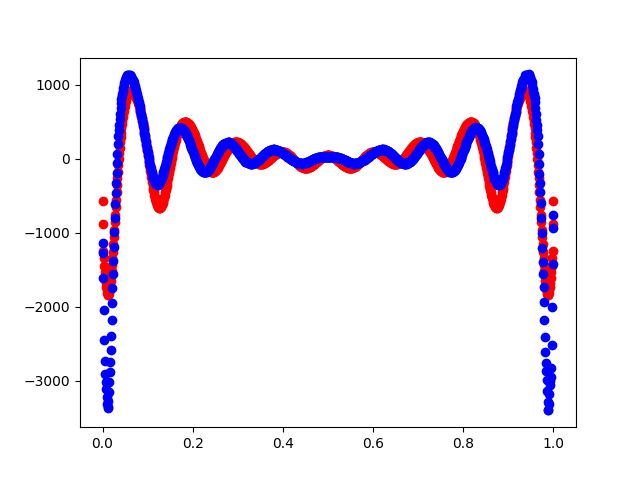
\includegraphics[width=6cm]{figure/example/model1_1000.png}
	\hspace{1cm}
	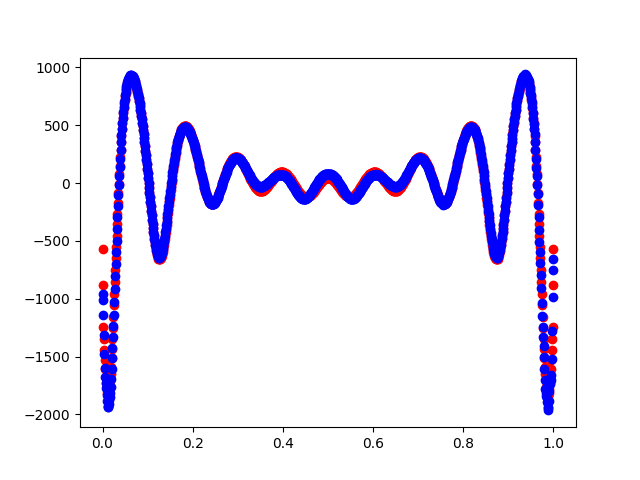
\includegraphics[width=6cm]{figure/example/model1_10000.png}
	\bicaption{中文题图}
	{English caption}
	\label{fig1}
\end{figure}

这里还有插入EPS图像和PDF图像的例子,如\autoref{fig2} 和\autoref{fig3}。这里将EPS和PDF图片作为子图插入,每个子图有自己的小标题。子图标题使用subcaption宏包添加。

\begin{figure}[htp]
	\centering
	\subcaptionbox{PDF 图像\label{fig2}}[3cm] %标题的长度,超过则会换行,如下一个小图。
	{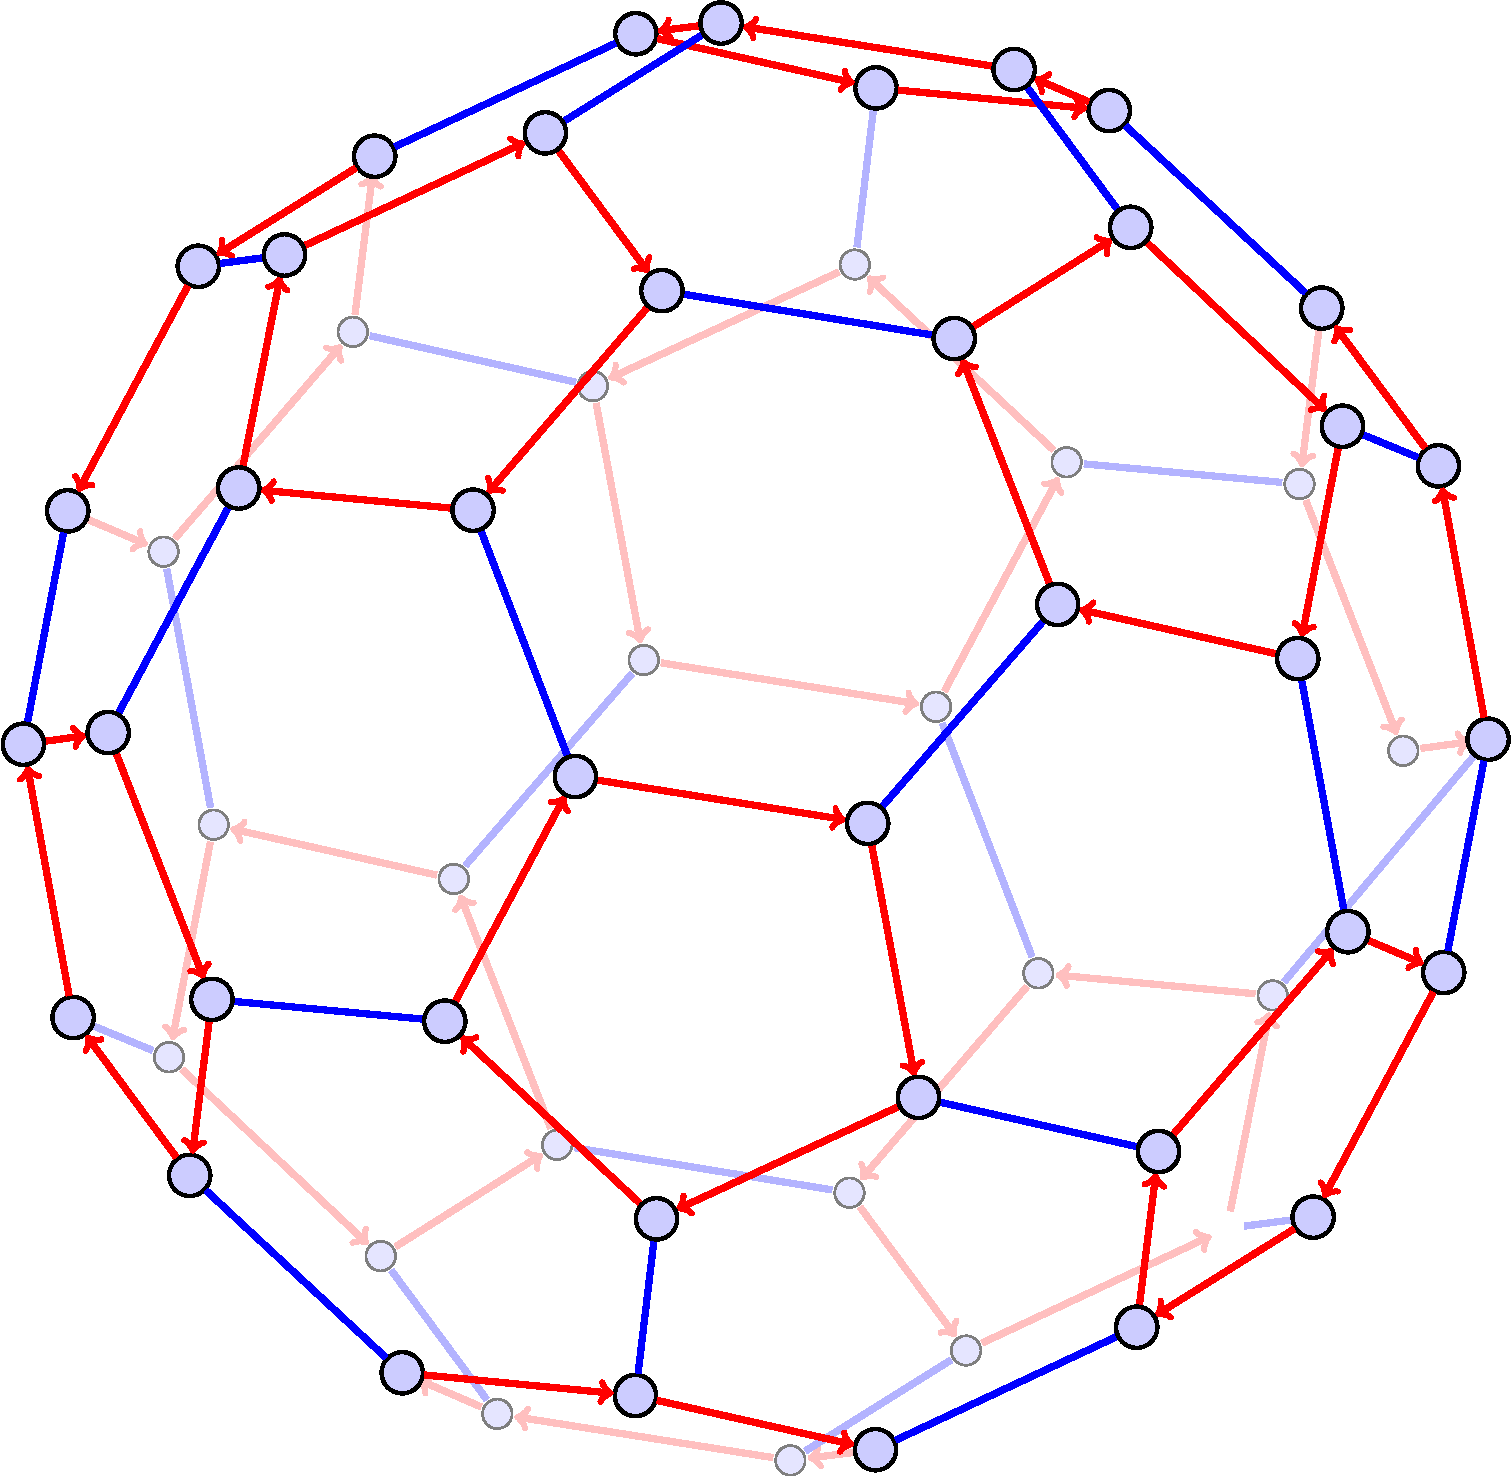
\includegraphics[height=2.5cm]{figure/example/m2.pdf}}
	\hspace{4em}
	\subcaptionbox{EPS 图像,如果标题很长的话,它会自动换行\label{fig3}}
	{	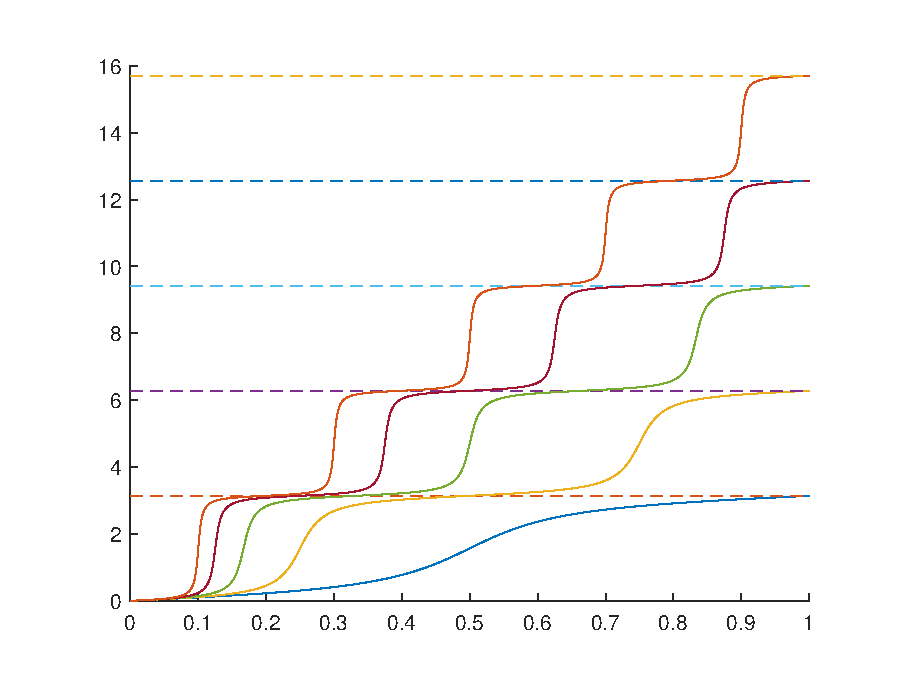
\includegraphics[scale=0.5]{figure/example/purfer_left.eps}}
	\bicaption{插入eps和pdf的例子(使用 subcaptionbox 方式)}{An EPS and PDF demo with subcaptionbox}
	\label{fig4}
\end{figure}。

\section{插入代码}

这里给一个使用listings宏包插入源代码的例子:
\begin{lstlisting}[language={C}, caption={一段C源代码}, label=code:1]
#include <stdio.h>

int main() {
    printf("Hello World!\n");
    return 0;
}
\end{lstlisting}
在\autoref{code:1}中,我们插入了一个C语言的Hello World代码。

\section{标签和引用}

这一节给出的是一些标签和引用的例子。

\subsection{标签设计原则}

为了更好的方便作者引用已经存在的标签,标签名必须见名知意。一般的设计原则是\verb|类型名:内容描述|。在\autoref{tab:typename} 中给出通常使用的类型的简称。

例如:\verb|thm:limit|,\verb|tab:typename|等等。

\begin{table}[!htp]
	\centering
	\caption{常见类型缩写}
	\begin{tabular}{c|c|c|c}\label{tab:typename}
		缩写 & 全称 & 缩写 & 全称 \\
		\hline
		part & part & fig & figure \\
		chap & chapter & tab & table \\
		sec & section & eq & equation \\
		subsec & subsection & algo & algorithm \\
		thm & theorem & def & definition \\
		lem & lemma & rem & remark \\
	\end{tabular}
\end{table}

\subsection{引用}

最简单的引用标签的方法就是使用\verb|\ref|命令,会显示被引用的定理(或者章节)对应的编号。
为了让文章可读性更强,我们通常会在\verb|\ref|命令前加入类型名,如\verb|<定理\ref{thm:telescope}>|。

\section{文献的添加和引用}

本模板的参考文献数据统一存放在\verb|bib/|目录下的\verb|ref.bib|文件中,如需添加文献,可以在INSPIRE HEP,百度学术,Google Scholar等界面查找到对应文献的\verb|bibtex|格式引用信息,然后附在\verb|ref.bib|文件末端即可。一个比较规范的\verb|bibtex|文献信息如下:
\begin{lstlisting}
@article{Sjostrand:2006za,
    author = "Sjostrand, Torbjorn and Mrenna, Stephen and Skands, Peter Z.",
    title = "{PYTHIA 6.4 Physics and Manual}",
    eprint = "hep-ph/0603175",
    archivePrefix = "arXiv",
    reportNumber = "FERMILAB-PUB-06-052-CD-T, LU-TP-06-13",
    doi = "10.1088/1126-6708/2006/05/026",
    journal = "JHEP",
    volume = "05",
    pages = "026",
    year = "2006"
}
\end{lstlisting}
第一行表明这个文献的类型是\verb|article|以及引用关键字为\verb|Sjostrand:2006za|。

文献添加后,如果需要引用,使用\verb|\cite{label}|命令即可,支持引用单个或多个文献。
演示如下:

命令\verb|\cite{Sjostrand:2006za}|的使用效果:在\cite{Sjostrand:2006za}中,作者已经阐述了有关结论。

命令\verb|\cite{bierlich2022comprehensive,王亚平2006}|的使用效果:在\cite{bierlich2022comprehensive,王亚平2006}中,作者有...

{\bf \textcolor{red}{重要提示}}:
如果在引用时发现不能正常显示引用标志的话,进入模板根目录下的\verb|cmd|环境,输入\verb|biber main|命令,然后再次编译即可。
   % 导入写作示例
% -*- coding=utf-8 -*-
\chapter{绪论}{绪论}    % \chapter{短标题}{长标题} 页眉会显示短标题,正文会显示长标题,“\\"会强制换行,”\ “会显示空格
我是绪论
\section{研究背景}
这样引用\cite{bierlich2022comprehensive}。如果ref.bib中的哪条参考文献没有在正文被引用,那么该条参考文献将不会在参考文献那一页显示出来。
\section{所做工作}       % 导入章节一
% -*- coding=utf-8 -*-
\chapter{预备知识}  % \chapter{短标题}{长标题} 页眉会显示短标题,正文会显示长标题,“\\"会强制换行,”\ “会显示空格
我是预备知识
       % 导入章节二                    % 载入章节内容
    \backmatter                                 	% 关闭章节序号,对页码没有影响
        \include{tex/6_reference}					% 载入参考文献
        \include{tex/7_appendix}                      % 载入附录
        \include{tex/8_thanks}           	% 载入致谢
\end{document}